\documentclass[11pt, a4paper]{article}

\usepackage[utf8]{inputenc}
\usepackage{graphicx}
\graphicspath{ {images/} }
\usepackage{mathtools}
\usepackage{amssymb}
\usepackage{amsmath}
\usepackage[ngerman,english]{babel}
\usepackage{cite}
\usepackage{bibgerm}
\usepackage{fullpage}
\usepackage[top=1.5cm,bottom=1.5cm,left=3.5cm,right=2.5cm,headsep=1.5cm,includeheadfoot]{geometry}
\usepackage{tabularx}
\usepackage{caption}
\usepackage{subcaption}
\usepackage{eurosym}
\usepackage{enumitem}
\usepackage{multicol}
\usepackage{tikz}
\usepackage{tkz-euclide}
\usepackage{pgfplots}
\usepackage{pdflscape}
\usepackage{acronym}
\usepackage{blindtext}
\usepackage{ifthen}
\usepackage{setspace}
\usepackage{cancel}
\usepackage{color}
\usepackage{listings}
\usepackage{comment}
\usepackage{xcolor}
\usepackage{colortbl}
\usepackage[parfill]{parskip}
\usepackage{url}

\usepackage{fancyhdr}
\pagestyle{fancy}

\fancyhf{} % clear all
\fancyhead[L]{\leftmark}
\fancyfoot[C]{-- \thepage{} --}
%\setlength{\headheight}{15pt}
\renewcommand{\headrulewidth}{0.5pt}
\renewcommand{\footrulewidth}{0pt}
\setlength{\skip\footins}{0.7cm}

\usetikzlibrary{graphs}
\usetikzlibrary{positioning}

\onehalfspacing
\setlength\parindent{0pt}

%\everymath{\displaystyle}

\allowdisplaybreaks

\definecolor{AI-BLUE}{rgb}{0,0.57,0.87}

% Eigene Befehle
\newcommand\q[1]{\glqq{}#1\grqq{}}
\renewcommand\equiv{\Leftrightarrow}
\newcommand\vertequal[2]{\underset{\underset{#2}{\parallel}}{#1}}
\newcommand\cif{\text{if }}
\newcommand\abs[1]{\left|#1\right|}
\newcommand\norm[1]{\abs{\abs{#1}}}
\newcommand\diff[1]{\text{ d#1}}
\newcommand\av[1]{\left\langle#1\right\rangle}
\newcommand\ev[1]{\mathbb{E}\left(#1\right)}
\newcommand\br[1]{\left(#1\right)}
\newcommand\ubr[2]{\underbrace{#1}_{#2}}
\newcommand\quer[1]{\overline{#1}}
\newcommand\setequal{\overset{!}{=}}
\newcommand\dint{\displaystyle \int}
\newcommand\dsum{\displaystyle \sum}
\newcommand\dprod{\displaystyle \prod}
\newcommand\closedInt[2]{\left[#1,#2\right]}
\newcommand{\checkbox}{\Large \Square \normalsize \hspace{0.4cm}}

\newcommand\myref[1]{\ref{#1} (S. \pageref{#1})}
\newcommand\myrefcomma[1]{\ref{#1}, S. \pageref{#1}}

\begin{document}

\thispagestyle{empty}

\setlength{\hoffset}{-0.5cm} % center title page

\lstset{
  basicstyle=\small,           % the size of the fonts that are used for the code
  breaklines=true,             % sets automatic line breaking
  captionpos=b,                % sets the caption-position to bottom
  frame=single,                % adds a frame around the code
  keepspaces=true,             % keeps spaces in text, useful for keeping indentation of code (possibly needs columns=flexible)
  numbers=right,               % where to put the line-numbers; possible values are (none, left, right)
  showspaces=false,            % show spaces everywhere adding particular underscores; it overrides 'showstringspaces'
  stepnumber=1,                % the step between two line-numbers. If it's 1, each line will be numbered
  tabsize=4,                   % sets default tabsize to 4 spaces
  xleftmargin=0.14cm		   % sets left margin
}


\begin{titlepage}
    \begin{center}
    \vphantom{0cm}
    \LARGE \textbf{Report}\\
    \vspace{3cm}
    \normalsize
    Study Project Report \\
    in the Master Program of \textcolor{AI-BLUE}{[Applied Computerscience]}\\
    at the Ruhr-University Bochum\\
    in the Winter Term 2015/16\\
    \vspace{4cm}
    \huge \textbf{Deep Convolutional Networks} \\
    \vspace{4cm}
    \normalsize
    \textbf{Project Participants}\\
    B. Sc. Christian Andreas Mielers (108 011 204 956)\\
    B. Sc. Phil Yannick Schrör (108 011 214 024)\\
    \vspace{2cm}
    \textbf{Project Supervisor:}\\
    PD Dr. Rolf P. Würtz
    \end{center}
\end{titlepage}

\newpage
\pagenumbering{arabic}
\setcounter{page}{2}

\tableofcontents

\newpage
\section{Introduction}
Convolutional neural networks (CNNs) are powerful tools in the field of machine learning. Their strength results from the efficient use of free parameters by exploiting the spatial structure of their input. Instead of learning every weight in the INPUT $\times$ OUTPUT matrix of a fully connected layer, a convolutional layer learns the weights in filters of a fixed size. Since the filters are generally tiny compared to a full weight matrix, using many filters and layers becomes feasible. The convolution operation with those filters then produces a layer response that indicates the local features represented by the filters.

To reduce the amount of data passed through the network, pooling layers that combine the values in small regions of the input into a single value can be used. One can then think of the consecutive application of convolutional and pooling layers as mechanisms to iteratively integrate features from ever more remote locations of the image into a compact representation. Fully connected layers can then be used on the representations learned by these layers to perform classification of the input.

Since images typically contain a lot of spatial structure, they are well suited for processing by such a CNN. To study and evaluate the properties of CNNs, we considered a network layout described in \cite{multi-column-neural-network-gtsrb}. Multiple networks which consist of three pairs of convolutional and pooling layers followed up with two fully connected layers were combined into a committee to solve the GTSRB challenge described in \cite{gtsrb}. We used the layout of one such network on the GTSRB dataset and two other datasets and measured the resulting accuracy. The filters on the various convolutional layers were visualized. We also transfered the filters learned on the GTSRB dataset to the other datasets and only trained the fully connected layers to evaluate how well they generalize.

\section{Network details}
The network layout we used is described in \cite{multi-column-neural-network-gtsrb} and summarized in table \ref{tab:network-layout}. It starts with a succession of 3 pairs of convolutional and max-pooling layers, where the number of filters increases with the depth of the network. The convolutions are executed such the output only consists of points for which all neccessary input values are available, and the max-pooling layers use non-overlapping regions to pool from. The convolutional-max-pooling pairs are followed by two fully connected layers, the latter of which has as many neurons as there are classes in the GTSRB dataset, suitable for one-hot encoding of class membership. Together with the notion that the first layer expects a 3-channel (RGB) image of size $48\times48$, the input and output sizes on all layers are determined.

\begin{table}[h!!!]
	\begin{tabular}{clll}
		Layer & Type & Configuration & Activation function \\
		\hline
		0 & Convolutional & 100 filters of size $7\times7$ per channel & $\tanh$ \\
		1 & Max Pooling & Pool size $2\times2$ & - \\
		2 & Convolutional & 150 filters of size $4\times4$ per channel & $\tanh$ \\
		3 & Max Pooling & Pool size $2\times2$ & - \\
		4 & Convolutional & 250 filters of size $4\times4$ per channel & $\tanh$ \\
		5 & Max Pooling & Pool size $2\times2$ & - \\
		6 & Dense & 300 neurons & $\tanh$ \\
		7 & Dense & 43 neurons & softmax
	\end{tabular}
	\caption{The layout of the network broken down by layer.}
	\label{tab:network-layout}
\end{table}

For all layers except the last one (and the max-pooling layers), a $\tanh$ activation function is used. The last layer uses a softmax activation to allow the interpretation of the output as class probabilities. All weights were uniformly initialized.

Training was performed by using stochastic gradient descent with an initial learning rate of $0.1$ and a decay of $1.0\times10^{-6}$ on the training data which was split into batches of $16$ images each. No momentum mechanism was used. The loss function optimized by the gradient descent was categorical crossentropy.

\section{Experiments with GTSRB}
The GTSRB dataset described in \cite{gtsrb} is a collection of $39209$ images in a training set and $12630$ images in a test set. In total, there are $43$ classes. The images were taken while driving through German streets and cropped to only contain the traffic sign and some boundary around it. For each physical traffic sign there are many images, that vary in distance, angle and occlusion since they were taken while the car was passing them. For each image, annotations exist, that locate the bounding box of the traffic sign. To generate fixed-size images for our network, we extracted only that part given by the bounding box and rescaled it to $48\times48$ pixels. As an additional preprocessing step, contrast normalization was applied to reduce the considerable illumination differences present in the images.

\subsection{Simple setup}
\label{subsec:simplesetup}
A network was trained on all images of the training set for $14$ epochs. On a TODO CPU with TODO RAM, one epochs takes about 10 hours. The performance development over the epochs is visualized in figure \ref{fig:gtsrb-results}, and the accuracy is given in a table. After achieving $\approx 0.9359$ after the first epoch, it rises monotonically and starts to levels off near $\approx 0.9640$ after about 6 epochs.

\begin{figure}[h!]
	\centering
	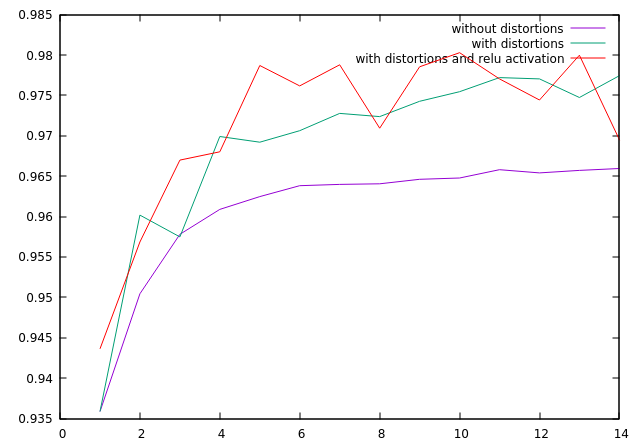
\includegraphics{gtsrb_results}
	\begin{tabular}{|r|rrr|}
		\hline
		Epoch & Simple setup & With distortions & With distortions (RELU) \\
		\hline
		1 & 0.9359 & 0.9359 & 0.9436 \\
		2 & 0.9504 & 0.9602 & 0.9568 \\
		3 & 0.9578 & 0.9575 & 0.9670 \\
		4 & 0.9609 & 0.9699 & 0.9680 \\
		5 & 0.9625 & 0.9692 & 0.9787 \\
		6 & 0.9638 & 0.9706 & 0.9762 \\
		7 & 0.9640 & 0.9728 & 0.9788 \\
		8 & 0.9641 & 0.9724 & 0.9709 \\
		9 & 0.9646 & 0.9743 & 0.9785 \\
		10 & 0.9648 & 0.9755 & 0.9803 \\
		11 & 0.9658 & 0.9772 & 0.9770 \\
		12 & 0.9654 & 0.9770 & 0.9744 \\
		13 & 0.9657 & 0.9747 & 0.9800 \\
		14 & 0.9660 & 0.9774 & 0.9695 \\
		\hline
	\end{tabular}
	\caption{Results of 3 network and training variants on the GTSRB test dataset. A network with a $\tanh$ activation function was trained on the data with and without distortions. Additionally, a network with the relu activation function was trained on the continually distorted data.}
	\label{fig:gtsrb-results}
\end{figure}

In the convolutional layers, the network learns filters that are applied to the 3 channels of the color image (in the lowest layer) and to the output of the previous layer (in later cases). Some of these filters are visualized in figure \ref{fig:gtsrb-filters}.

One can observe that the filters on the first layer exhibit a notable spatial structure. In most of them, we see rather broad regions that contain either high or low values. Due to this, one can easily see how they work as feature detectors for the network. They seem to be tuned for edges and corners of various orientations, since this is what the shape of the borders between bright and dark regions mostly suggest. It is also striking that the filters for the 3 channels share a common layout, save for a few details. This indicates that the first layer combines the channels into a unified representation without discriminating between colors. Thus, it seems that the network learns to classify the traffic signs without a lot of dependence on color information.

The filters on the higher layers are not so easy to reason about. They have less room to expose structure since they are smaller, but even so there doesn't seem to be a separation between regions of high and low values as distinct as on the lowest layer. Since there are a lot of filters for every one of the many input maps to those layers, there is a sizable number of filters involved. This high number of filters might make it useful to increase the specialization of those filters, leading to structures that do not correspond to a visually striking layout.

\begin{figure}
	\centering
	\begin{subfigure}{\textwidth}
		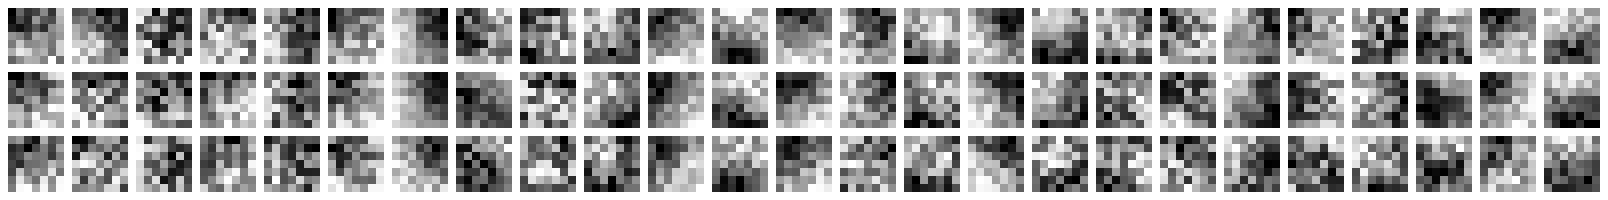
\includegraphics[width=1\textwidth]{filter_visualizations/gtsrb_nomorph_filters_0}
		\caption{Layer 0}
		\label{fig:gtsrb-filters-0}
	\end{subfigure}
	\begin{subfigure}{\textwidth}
		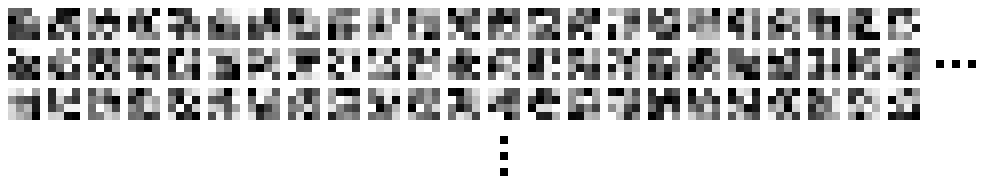
\includegraphics[width=1\textwidth]{filter_visualizations/gtsrb_nomorph_filters_2}
		\caption{Layer 2}
		\label{fig:gtsrb-filters-2}
	\end{subfigure}
	\begin{subfigure}{\textwidth}
		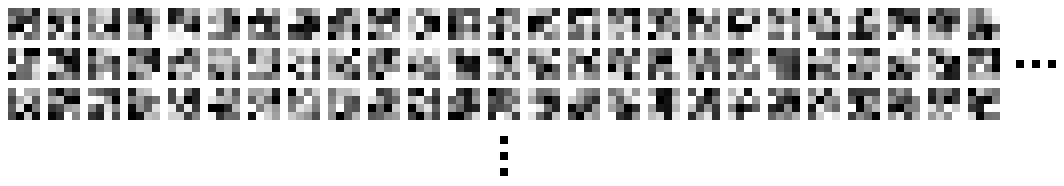
\includegraphics[width=1\textwidth]{filter_visualizations/gtsrb_nomorph_filters_4}
		\caption{Layer 4}
		\label{fig:gtsrb-filters-4}
	\end{subfigure}
	\caption{Filter visualization for the network trained on the original input data after 14 epochs. (\subref{fig:gtsrb-filters-0}): Filters of the first 25 maps from the first convolutional layer. The three rows show the filters for the red, green and blue channel respectively. (\subref{fig:gtsrb-filters-2}) and (\subref{fig:gtsrb-filters-4}): First few filters for the first 25 maps of the second and third convolutional layers, respectively.}
	\label{fig:gtsrb-filters}
\end{figure}

\subsection{Input distortions}
\label{subsec:inputdistortions}

An additional technique used in \cite{multi-column-neural-network-gtsrb} is the distortion of input data. In order to help the network generalize better from the given training set, slight distortions were applied to each input image between epochs. These distortions comprise rotation, scaling and translation. The details are found in section \ref{sec:implementation-distortions}.

As one can see in figure \ref{fig:gtsrb-results}, this significantly boosted the performance. After 14 epochs, the network that was trained on the distorted images achieved a success rate about $1.1$\% higher, with an accuracy of $\approx 0.9774$\%. Overall, the curve is a bit more volatile than the one without distortions. This might indicate that the distortions influence the network quite strongly and weaker transformation parameters may lead to steadier learning, but more training rounds would be neccessary to be certain of this.

Visual inspection of the convolutional filters shows that they are not qualitatively different from those in \ref{fig:gtsrb-filters}. As before, the first layer exhibits a visible spatial structure with regions of high and low values. Their shape suggests their role as edge and corner detectors. Again, the filters for all 3 channels share their general appearance, suggesting mostly color independence. On the other convolutional layers, the possibility of visual interpretation is small, just as before.

\subsection{RELU activation function}
The layers in \cite{multi-column-neural-network-gtsrb} used a $\tanh$ activation function. For performance reasons the RELU activation function, as shown in figure \ref{fig:relu} is often used as a fast-to-compute alternative that yields good results.

\begin{figure}[h!!!]
	\centering
	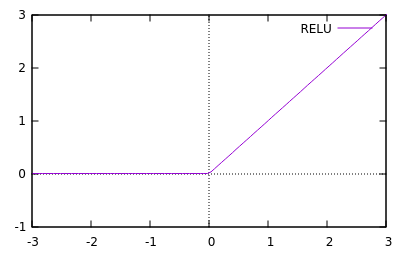
\includegraphics{images/relu.png}
	\caption{RELU activation function}
	\label{fig:relu}
\end{figure}

To examine the influence of the choice of activation function, we trained the same network from table \ref{tab:network-layout} from the ground up. The only difference to the old network was the usage of the RELU activation function instead of $\tanh$. Since distortions proved effective, they were again used in this training run. The accuracy over 14 epochs is shown in \text{figure \ref{fig:gtsrb-results}}.

One can observe that this network accomplishes a considerably higher performance than the one with the original $\tanh$ activation function at certain points. The $\tanh$ network reaches its peak of $\approx 0.9774$\% accuracy after 14 epochs, while the RELU network peaks at $\approx 0.9803$ after 10 epochs. However, its behavior over the course of training is much more volatile. Epochs where the performance is superior to the $\tanh$ network are interspersed with drops below $\tanh$ performance. More trials would be neccessary to be sure, but it seems that a RELU activation behaves less predictable during training.

\subsection{Misclassified images}
Useful insights may be gained by looking at the errors that a network makes. To this end, we considered the misclassified images in the test set and looked at the 3 most likely classes predicted by the network. The network with RELU activation has achieved the highest accuracy overall, but since its performance as proven unreliable, we visualized the errors made by the $\tanh$ network after 14 epochs with distorted input data.

\begin{figure}
	\centering
	\begin{subfigure}{\textwidth}
		\centering
		\caption{}
		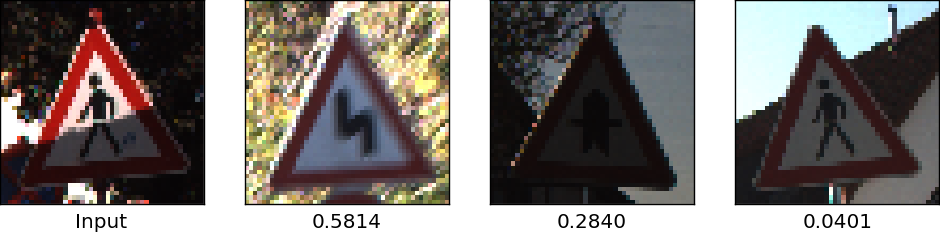
\includegraphics[width=0.7\textwidth]{gtsrb_mistakes/mistake_fussgaenger.png}
		\label{fig:gtsrb-mistakes-01}
	\end{subfigure}
	\begin{subfigure}{\textwidth}
		\centering
		\caption{}
		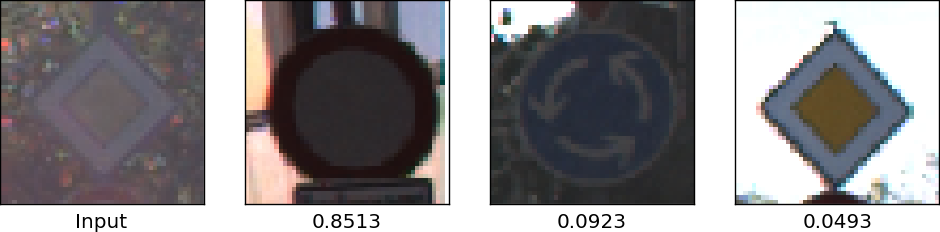
\includegraphics[width=0.7\textwidth]{gtsrb_mistakes/mistake_vorfahrtstrasse.png}
		\label{fig:gtsrb-mistakes-02}
	\end{subfigure}
	\begin{subfigure}{\textwidth}
		\centering
		\caption{}
		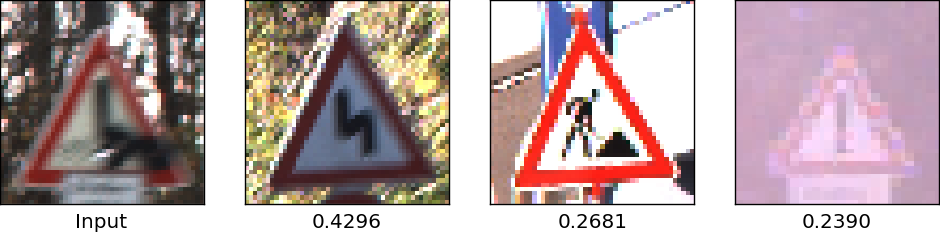
\includegraphics[width=0.7\textwidth]{gtsrb_mistakes/mistake_gefahrenstelle.png}
		\label{fig:gtsrb-mistakes-03}
	\end{subfigure}
	\begin{subfigure}{\textwidth}
		\centering
		\caption{}
		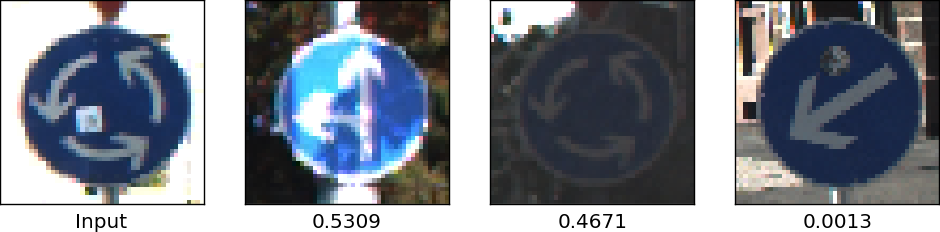
\includegraphics[width=0.7\textwidth]{gtsrb_mistakes/mistake_kreisverkehr.png}
		\label{fig:gtsrb-mistakes-04}
	\end{subfigure}
	\begin{subfigure}{\textwidth}
		\centering
		\caption{}
		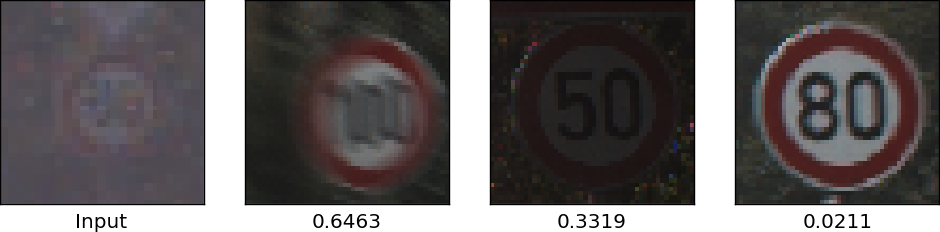
\includegraphics[width=0.7\textwidth]{gtsrb_mistakes/mistake_limit_unknown.png}
		\label{fig:gtsrb-mistakes-05}
	\end{subfigure}
	\begin{subfigure}{\textwidth}
		\centering
		\caption{}
		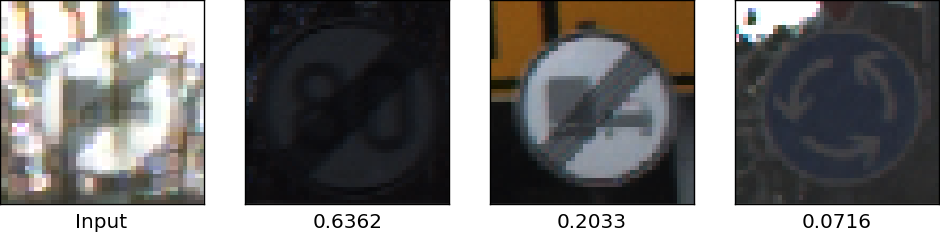
\includegraphics[width=0.7\textwidth]{gtsrb_mistakes/mistake_ueberholen_lkw.png}
		\label{fig:gtsrb-mistakes-06}
	\end{subfigure}
	\begin{subfigure}{\textwidth}
		\centering
		\caption{}
		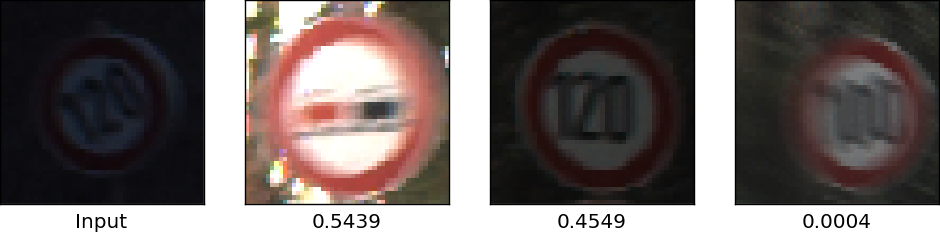
\includegraphics[width=0.7\textwidth]{gtsrb_mistakes/mistake_limit_120.png}
		\label{fig:gtsrb-mistakes-07}
	\end{subfigure}
	\caption{Selected misclassified images of the network with $\tanh$ activation and distorted input data after 14 epochs. Additionally, the 3 most likely candidates predicted by the network are shown together with their probabilities.}
	\label{fig:gtsrb-mistakes}
\end{figure}

An accuracy of $0.9774$\% on a test set with 12630 images implies 285 misclassifications. Most of those instances come from a handful of traffic signs (since there are multiple images of each pyhsical sign). Hand-selected examples of these instances are shown in figure \ref{fig:gtsrb-mistakes}. Although the predicted probabilities can be quite high, they are significantly lower than the predicted probabilities for correctly classified images, which are usually above $95$\%.

Some of the errors seem quite avoidable. For instance, a human could easily classify \ref{fig:gtsrb-mistakes-01} and \ref{fig:gtsrb-mistakes-02}. While the network sticks to triangular traffic signs for \ref{fig:gtsrb-mistakes-01}, it is willing to predict round signs for the rectangular input in \ref{fig:gtsrb-mistakes-01}. In this example, it is also clear that the color of the sign is not crucial for the prediction, as red and blue signs are predicted while the input contains a yellow region.

Other possible causes for misclassification are depicted in \ref{fig:gtsrb-mistakes-03} and \ref{fig:gtsrb-mistakes-04}. Here, shape and color of the predictions match those of the input. The error can be attributed to occlusion occuring on the input, but in both cases a human would stand a reasonable chance to identify the traffic sign.

Figures \ref{fig:gtsrb-mistakes-05} and \ref{fig:gtsrb-mistakes-06} show cases that are somewhat hopeless. Although the former appears to be a speed limit sign and the latter is similar to prediction 2, one can not really be certain by just inspecting the image. A last notable example is \ref{fig:gtsrb-mistakes-07}. Here we see a strongly tilted speed limit sign. It is understandable that this complicates the task, although the distortions applied during training should have induced a slight rotation invariance. It would be interesting to see whether stronger training data distortions would prevent misclassifications like these.

\section{Filter reuse}

In order to examine how well the convolution filters trained on the GTSRB dataset generalize, we used the GTSRB filters also on other datasets. After several epochs of training on the GTSRB dataset, we copied the weights of the convolutional layers to another CNN and trained only the randomly initialized weights of fully-connected layers in the new network. Thus, the weights of the convolutional layers, i.e. the filters, remained unchanged. To evaluate how well this approch works in terms of training time and classification results, we also trained the weights of all layers completely from scratch on these other datasets and compared the results. Those filters trained from the ground up will be called \textit{original} filters in the following considerations, since they are original to this very classification task and classifier.

\subsection{COIL100 dataset}

The first dataset we used is the COIL100 (Columbia Object Image Library 100) dataset (cf. \cite{columbia_object_image_library}), which contains images of 100 different objects. Figure \ref{fig:coil100_objects} shows a subset of 20 objects out of the whole dataset. Each object constitutes one class, hence, it is a classification problem with 100 classes. The individual objects were placed on a black turntable in front of a black background. 
\begin{figure}[h!]
	\centering
	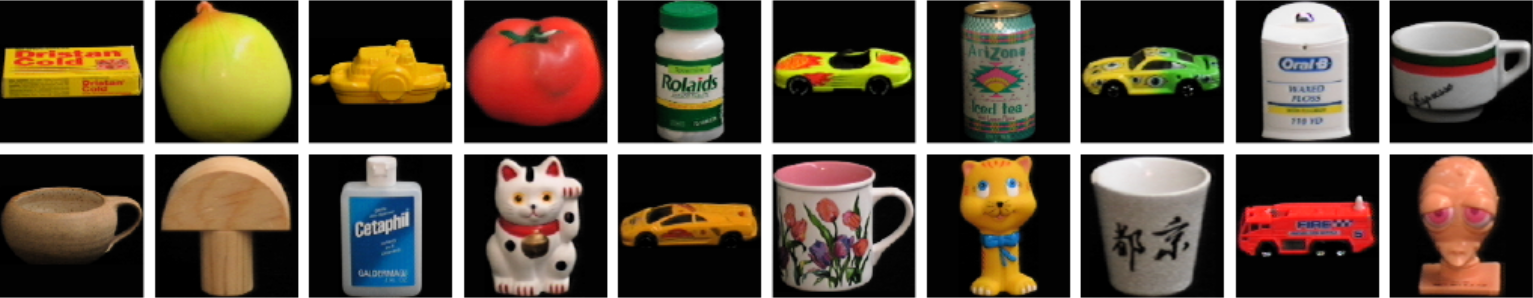
\includegraphics[width=1\textwidth]{coil100}
	\caption{A subset of 20 objects taken from the COIL100 dataset.}
	\label{fig:coil100_objects}
\end{figure}
In order to be able to present the learning algorithm many different views on one single object, the camera took a photo of the rotating object, each time it has turned by 5 degrees, yielding 72 images per object and 7200 images in total. Since the creators of the dataset do not provide or suggest any established separation into training and test data, we created those sets on our part, randomly dividing the 72 images of each object into 58 training images and 14 test images, totaling in 5800 training and 1400 test images.\\
Since the provided images are already cropped in a reasonable manner, unlike the images of the GTSRB dataset, we did not crop the images any further. However, we were obliged to rescale the images to a size of $48 \times 48$ pixels to fit the structure of the adopted GTSRB CNN; otherwise we would not have been able to reuse the filters trained on the GTSRB network, because their sizes would not match those of the filters of the COIL100 network. Since we had found that distorting the images before each training epoch had improved the results on the GTSRB dataset, we applied the distortions also to the images of the COIL100 dataset.

\subsubsection{Results with reused GTSRB filters}

The curve "Reused GTSRB filters" in figure \ref{fig:coil100_results} illustrates the results on the test set, which we achieved by letting the weights of the convolutional layers unchanged and training only the randomly initialized weights of the fully connected layers. The column "GTSRB filters" in table \ref{tab:coil-results} provides the exact numbers rounded to the fourth decimal place. We observe that the accuracy increases monotonically until the eighth epoch, where we obtained a result of 100\%. The following slight decrease of the recognition rate can be explained as a consequence of the randomized distortions, which are applied before each epoch. Howsoever, the accuracy does not decrease by a large amount (an accuracy of 99.93\% indicates one misclassfied image, 99.79\% indcate three misclassified images) and stabilizes again at 100\% after 14 epochs. Training one epoch lasts about 300 seconds on the given hardware configuration. Thus, it is possible to construct a reliable classifier for this task in a short time interval by reusing pre-trained filters from another network.%TODO Add information about zappa02 processor ecc.

\begin{figure}[h!]
	\centering
	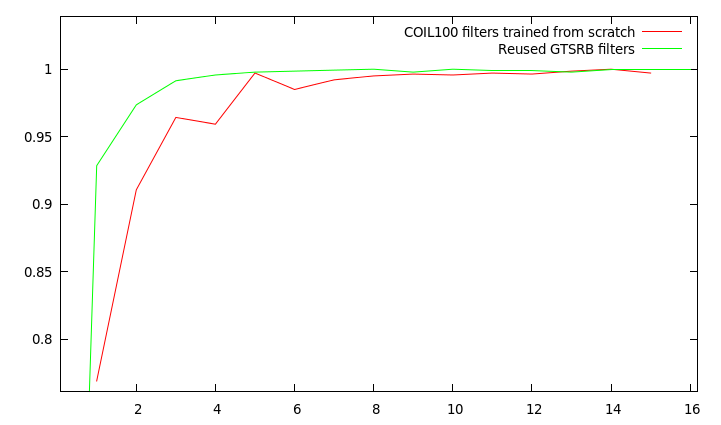
\includegraphics[width=1\textwidth]{coil100_results.png}
	\caption{Results on COIL100 with original filters and with reused GTSRB filters.}
	\label{fig:coil100_results}
\end{figure}
\begin{table}[h!]
	\centering
	\begin{tabular}{|r|rr|}
		\hline
		Epoch & GTSRB Filters & Original Filters\\ \hline
		00 & 0.0250 & -\\
		01 & 0.9286 & 0.7693\\
		02 & 0.9736 & 0.9107\\
		03 & 0.9914 & 0.9643\\
		04 & 0.9957 & 0.9593\\
		05 & 0.9979 & 0.9971\\
		06 & 0.9986 & 0.9850\\
		07 & 0.9993 & 0.9921\\
		08 & 1.0000 & 0.9950\\
		09 & 0.9979 & 0.9964\\
		10 & 1.0000 & 0.9957\\
		11 & 0.9993 & 0.9971\\
		12 & 0.9993 & 0.9964\\
		13 & 0.9979 & 0.9986\\
		14 & 1.0000 & 1.0000\\
		15 & 1.0000 & 0.9971\\ \hline
	\end{tabular}

	\caption{Results on COIL100 with reused GTSRB filters and original filters.}
	\label{tab:coil-results}
\end{table}

\subsubsection{Results with original filters}

In addition, we set up a network with the same structure, but initialized the weights of all layers randomly. The results of this setup are illustrated by the curve "Original COIL100 filters" in figure \ref{fig:coil100_results} and the column "Original Filters" in table \ref{tab:coil-results}. After some fluctuations during the first few epochs, the recognition rate does not exhibit larger variations and yields reliable results. In spite of the fact that the accuracy curve of the original filters is dominated by the curve of the GTSRB filters for the first 12 epochs, we observe that the results with the original filters eventually reach the same level as those of the GTSRB filters do.\\
A clear disadvantage of training original filters is the extensively larger training time of approximately 5300 seconds, which are required to train the network for a single epoch. This is the time, which is needed to train only the weights of the fully connected layers for one epoch, multiplied by a factor of about 17.\\
In chapter \ref{subsec:simplesetup} we pointed out that the filters of the first convolutional layer of the \text{GTSRB} network exhibit a clear spatial structure, which led us to the assumption that those filters may be sufficiently generalized to provide solid results on other datasets, too. The results achivied by using the GTSRB filters on the COIL100 dataset seem to confirm this assumption. The comparison between the filters of the first convolutional layer of the GTSRB network and those of the same layer in the COIL100 network presented in \text{figure \ref{fig:gtsrb_vs_coil_filters}} reveals that the same assumption cannot be made for the COIL100 filters. In spite of the fact that there are some filters (e.g. those in the 5th and 17th column), which bear resemblance to the GTSRB filters, the overall structure appears much more noisy and less meaningful. This leads to the conclusion that the COIL100 network is overfitted to this very problem and does not extract meaningful features, which could be used for other classification tasks on different datasets. These findings do not necessarily exclude the possibility that a reasonable set of filters can be constructed by training a CNN on the COIL100 dataset. It is probable that the network used in this experiment is just too oversized for a rather easy problem like the classification task on the COIL100 dataset. In a further consideration one could train a CNN with a more appropriate structure on the COIL100 dataset, which does not need fo fulfill the constrains imposed by the GTSRB network.\\
In contrast to the GTSRB filters, which exhibit a very similar filter structure for all three color channels, the original filters appear to be more color dependent. Although we do find some filter triples, which show areas of large values and of small values at virtually the same positions, there are also many filters with quite diverse patterns for the different channels (e.g. those column 14). Given that the COIL100 objects are colored very differently, it seems logical to base the classification decision also on the available color information.

\begin{figure}[h!]
	\centering
	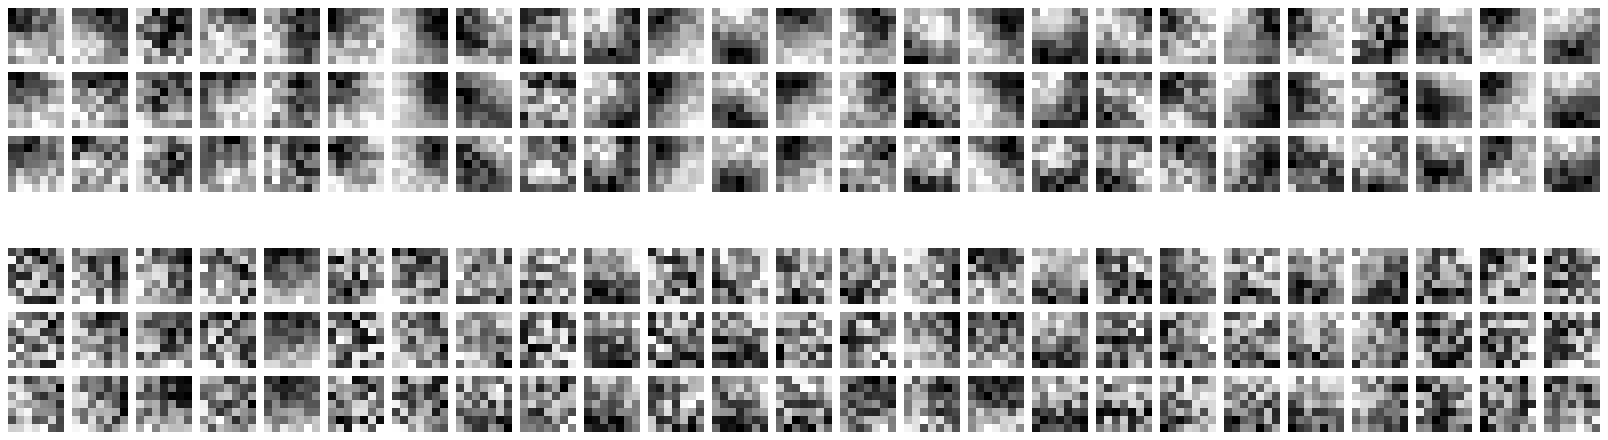
\includegraphics[width=1\textwidth]{gtsrb_vs_coil_filters.png}
	\caption{Filters of the first 25 maps from the input layer to the second layer. The upper filters are taken from the GTSRB CNN after 12 epochs of training, the lower filters are taken from the COIL100 CNN after 15 epochs of training. The three rows show the filters for the red, green and blue channel respectively.}
	\label{fig:gtsrb_vs_coil_filters}
\end{figure}


\subsection{INRIA dataset}
\label{subsec:inria}

After achieving excellent results with the GTSRB filters on the COIL100 dataset, we tried to get similar results on a probably more difficult dataset in order to alleviate the probability of having achieved our results only owing to unfortunate circumstances like noise or a too simple problem. The dataset we chose is the Head Pose Image Database \cite{estimating-face-orientation-inria} from the French Institute for Research in Computer Science and Automation (INRIA). The dataset consists of 15 persons, 2 series per person and 93 JPEG-images per series. In each series the depicted person changes its head posture gradually. Often one of the two series shows the person with a certain feature like glasses, while the other series does not. Since there is not given a fixed seperation into training and test data, we randomly splitted the 186 images per person into 149 training and 37 test images, ignoring to which series an image belongs. Figure \ref{fig:inria_different_angles} presents a subset of images taken from one series for one person.

\begin{figure}[h!]
	\centering
	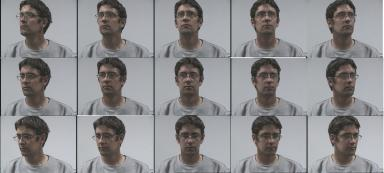
\includegraphics[width=0.8\textwidth]{inria_different_angles}
	\caption{Several head positions of person 12 with glasses.}
	\label{fig:inria_different_angles}
\end{figure}

The problem appears to be harder than the COIL100 problem, because the persons in the INRIA dataset are more similar to each other than the objects in the COIL100 dataset. For instance, the persons are not well distinguishable by color, given that all persons have a similar hair and a similar skin color. Hence, the network will most likely not assemble filters for the first layer, which differ a lot for the three single color channels.\\
Even if the images of this dataset have a larger margin than the images of the GTSRB and COIL100 datasets, we did not define a bounding box to crop off the probably unneccessary information from the images. Nonetheless we achieved acceptable results.

\subsubsection{Reused GTSRB filters}

The curve "Reused GTSRB filters" in figure \ref{fig:inria_results} and the column "GTSRB Filters" in table \ref{tab:inria-results} illustrate the test results of a CNN trained on the INRIA dataset. As we did for the COIL100 dataset, we took also for this network the weights of the convolutional layers of the GTSRB network after a training time of 12 epochs. Again, the weights of the fully-connected layers were initialized randomly and then trained until an adequate recogniton rate was obtained.

\begin{figure}[h!]
	\centering
	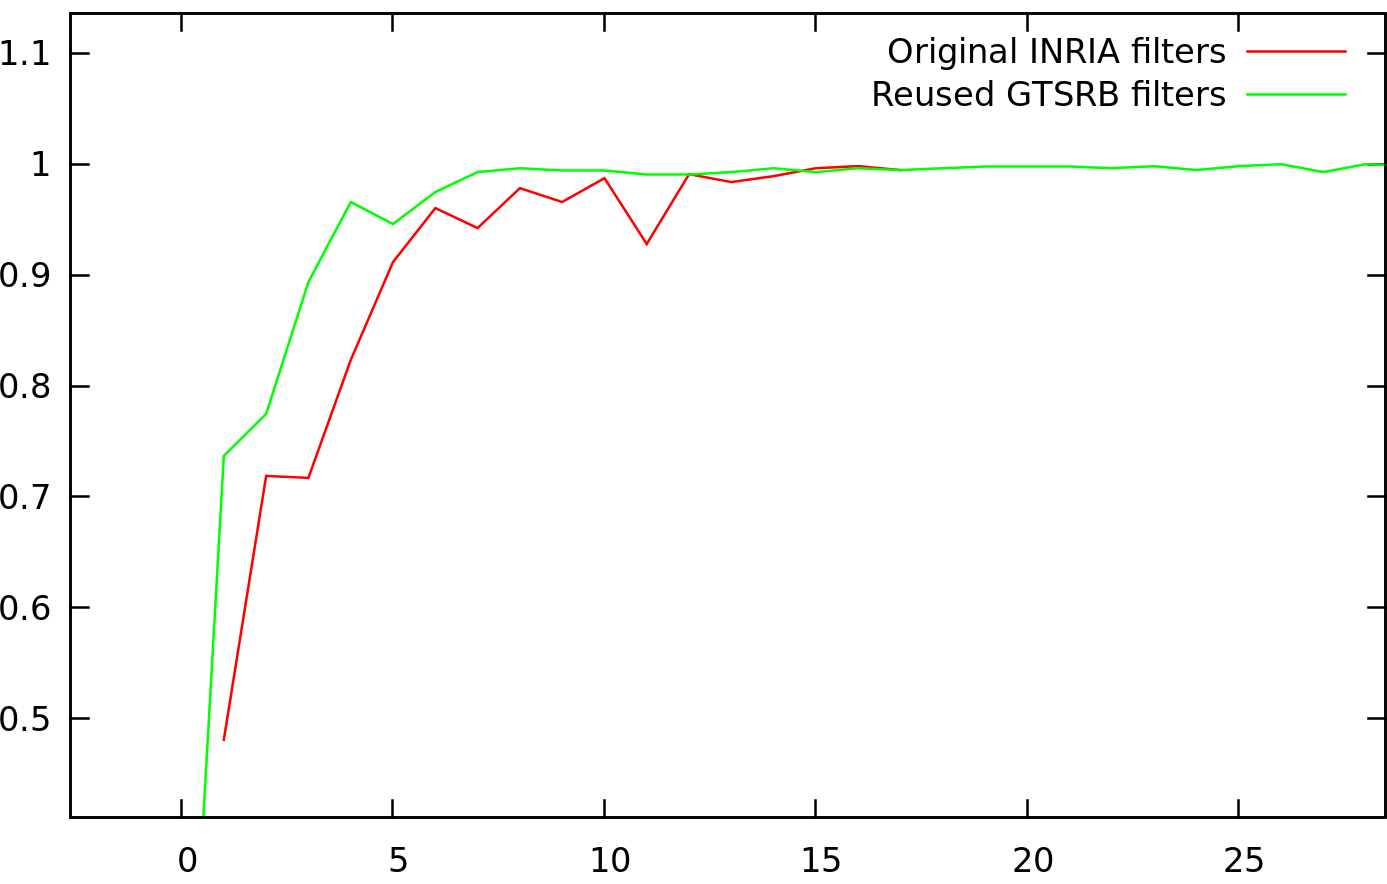
\includegraphics[width=1\textwidth]{inria_results.png}
	\caption{Results on the INRIA dataset with original filters completely trained from the ground up and with reused GTSRB filters.}
	\label{fig:inria_results}
\end{figure}

Very good results are reached after only a small number of epochs. After 7 epochs, an accuracy of above 99\% is obtained for the first time. Again, the fluctuation of the recognition rate can be explained as a consequence of the random distortions, which are applied before each training epoch. Owing to the short training time, the network was trained in total for 60 epochs with the GTSRB filters. We observed that the accuracy fell only 3 times below a value of 99.5\% after training the network for 20 epochs. Furthermore we reached several times a recognition rate of 100\% (for the first time in epoch 26), but could not keep it for more than 4 epochs in a row.
A consequence of having only $186 \cdot 15 = 2790$ images in total and $(186 - 37) \cdot 15 = 2235$ training images is the fact that training the fully-connected layers for one epoch does not even require 2 minutes (depending on the used hardware).

\begin{table}[h!]
	\centering
	\begin{tabular}{|r|rr|}
		\hline
		Epoch & GTSRB Filters & Original Filters\\ \hline
		00 & 0.0667 & -\\
		01 & 0.7369 & 0.4811\\
		02 & 0.7748 & 0.7189\\
		03 & 0.8937 & 0.7171\\
		04 & 0.9658 & 0.8234\\
		05 & 0.9459 & 0.9117\\
		06 & 0.9748 & 0.9604\\
		07 & 0.9928 & 0.9423\\
		08 & 0.9964 & 0.9784\\
		09 & 0.9946 & 0.9658\\
		10 & 0.9946 & 0.9874\\
		11 & 0.9910 & 0.9279\\
		12 & 0.9910 & 0.9910\\
		13 & 0.9928 & 0.9838\\
		14 & 0.9964 & 0.9892\\
		15 & 0.9928 & 0.9964\\
		16 & 0.9964 & 0.9982\\
		17 & 0.9946 & 0.9946\\ \hline
	\end{tabular}

	\caption{Results on INRIA with reused GTSRB filters and original filters. }
	\label{tab:inria-results}
\end{table}

Hence, we find one more time, that it is possible to construct a CNN for such a classification problem in a comparatively short time interval by copying the apparently sufficiently generalized filters from another network trained on another dataset to a new network and then training only the fully-connected layers.

\subsubsection{Original filters}

After having found that the GTSRB filters work well on the INRIA dataset, we trained another CNN on this dataset without copying any weights. All weights were randomly initialized and then trained for 17 epochs, yielding the results presented by the curve "Original INRIA filters" in \text{figure \ref{fig:inria_results}} and the column "Original filters" in table \ref{tab:inria-results}.\\
As already observed for the original COIL100 filters, also the results for the original INRIA filters are dominated by the results obtained by using the GTSRB filters on the INRIA dataset. Epoch 15 is the first epoch, which shows a better result for the original filters (99.64\%) than for the GTSRB filters (99.28\%).\\
With regard to the training time, which is required to train the networks of the two different approaches (copying or not copying the GTSRB weights), it can be stated that it demands much more time to train the network, which trains all weights of all layers. It takes over 2000 seconds to train the network including the convolutional filters and a little less than 120 seconds to train the network, which instead relies on the GTSRB filters. This is (as it was for the COIL100 networks) a factor of around 17. So it does not pay off to train a complete network without reused weights in order to yield better results. Quite the contrary, better results in the beginning and approximately equally good results after a certain amount of epochs are obtained in a less expensive way with regards to the training time by reverting to previously trained weights.\\
For the COIL100 original filters we found that they were not well-structured and comprised a lot noise. The original INRIA filters, on the other hand, reveal a structure as easily interpretable as the GTSRB filters. \text{Figure \ref{fig:gtsrb_vs_inria_filters}} opposes the GTSRB filters to the original INRIA filters, demonstrating that there is no perceivable qualitative difference between the two filter sets. The filters of both networks should work well as edge and corner detectors and should be largly interchangeable (training a CNN with the original INRIA filters on the COIL100 dataset yielded a result of 99.79\% on the test dataset after 10 epochs). Since one epoch takes around 10 hours for the GTSRB network and only around half an hour for the INRIA network, this is a relevant finding.
%TODO ADD RESULTS


\begin{figure}[h!]
	\centering
	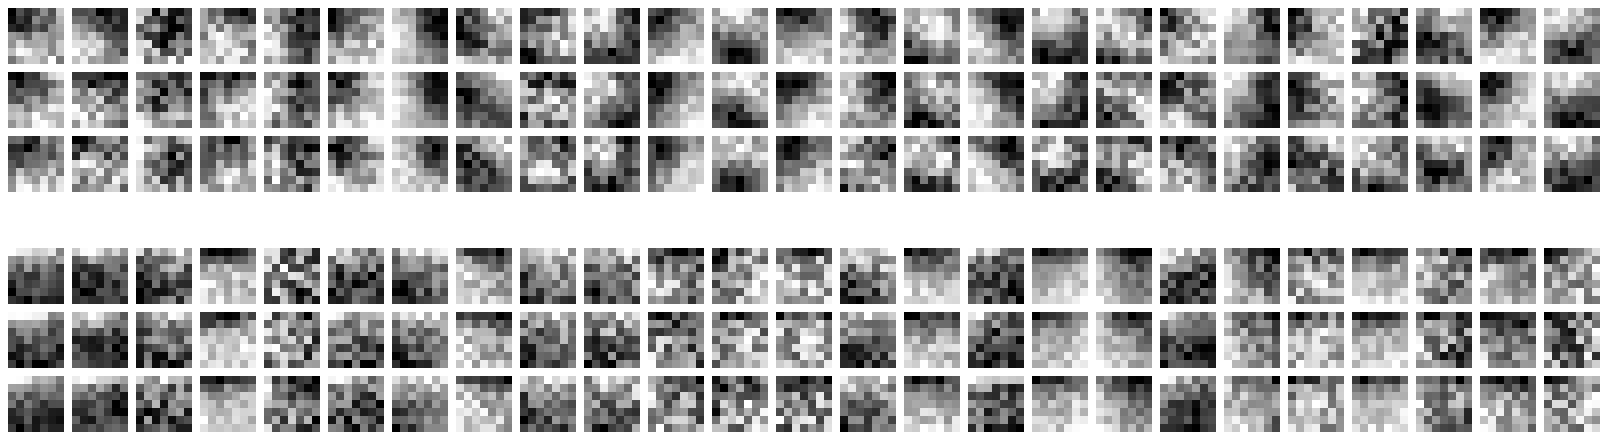
\includegraphics[width=1\textwidth]{gtsrb_vs_inria_filters.png}
	\caption{Filters of the first 25 maps from the input layer to the second layer. The upper filters are taken from the GTSRB CNN after 12 epochs of training, the lower filters are taken from the INRIA CNN after 17 epochs of training.}
	\label{fig:gtsrb_vs_inria_filters}
\end{figure}

As expected before training the original filters, the filters in one filter triplet for the 3 color channels are very similar to each other and differ only in rare cases. This observation reaffirms the expectation that the filters work mostly color independent and put much more confidence in the geometrical shape of the images.\\
Finally it can be stated that not only the training on the GTSRB dataset but also the training on the INRIA dataset produces reasonable filters, which can actually be reused in other networks to solve other classifcation tasks.


\section{Conclusion}


\begin{appendix}
	\section{Implementation}
	
	\subsection{Neural Network}
	For the technical realization of the network, we used the \emph{Keras} neural network library for the \emph{Python} programming language. Initially, we tried the \emph{Sharkonvnet} extension for the \emph{Shark} machine learning \emph{C++} library, but realized that it is far from finished. A next option was the \emph{Caffee} neural network \emph{C++} library. This seemed like a versatile and efficient option. However, for its network definitions it relies heavily on the \emph{Google Protobuf} protocol definition standard which would have required a large effort to familiarize with, disproportional to the time available for a study project.
	
	\subsection{Distortions}
	\label{sec:implementation-distortions}
	% TODO be precise about the input being distorted before the first epoch.
	As already hinted at in chapter \ref{subsec:inputdistortions}, all training images are distorted before each epoch.
	One should notice that the images are already rescaled to the size $a \times b$, which is defined in the layout file for the respective network, before the transformations are applied.\\
	Firstly, the image is shifted horizontally by $x \sim \mathcal{U}(- 0.1 w, 0.1 w)$ pixels and vertically by $y \sim \mathcal{U}(- 0.1 h, 0.1 h)$ pixels with $w$ as width and $h$ as height of the image. In a second step, the image is rotated by $r \sim \mathcal{U}(-5, 5)$ degrees. As third transformation a scaling by a factor $s \sim \mathcal{U}(0.9,1.1)$ is applied to the image.\\
	After applying the distortions, the images are cropped to the correct size. If the image is larger than required, the cropping frame is centered in the middle of the image and the borders are dismissed. If the images is smaller than required, pixels are added to all four sides of the image. Those pixels are filled with the grayvalue of the closest pixel of the original image after the transformation.\\
	Lastly it must be mentioned that the distorted images are dismissed after finishing one epoch, so that the distortions are always applied to the original images (rescaled to the required size $a \times b$). Otherwise the images would be too distorted after a few epochs and further training would become impractical.
	
	\section{Visualization}
\end{appendix}

\addcontentsline{toc}{section}{References}
\bibliography{ref}{}
\bibliographystyle{alpha}

\end{document}






